%Background body
%Created MS 05-11

\section{Background}\label{background}

\subsection{Optical Pumping}\label{opticalpumping}

Optical pumping is the process in which the interaction of light with
atoms produces a population of energy levels that is distinct from the
thermal equilibrium Boltzmann distribution \cite{bernheim}. In a
three-state system, with a ground state $|g\rangle$, excited state
$|e\rangle$, and intermediate metastable state $|m\rangle$
(Fig. \ref{fig:pumping}), it is possible to selectively populate the metastable
state if the natural decay time $\gamma_{rel}$ is sufficiently long in
comparison to the pumping time. If laser light is applied on resonance
with the $|e\rangle$ to $|g\rangle$ transition, it drives the atom
population to the excited state, and then the atoms decay to the lower
energy levels with some time constant. If the laser light cannot
excite atoms from the metastable state to the excited state (for
example, due to selection rules), the process preferentially populates
the state $|m\rangle$, resulting in optical pumping.


\begin{figure}[h]
\begin{center}
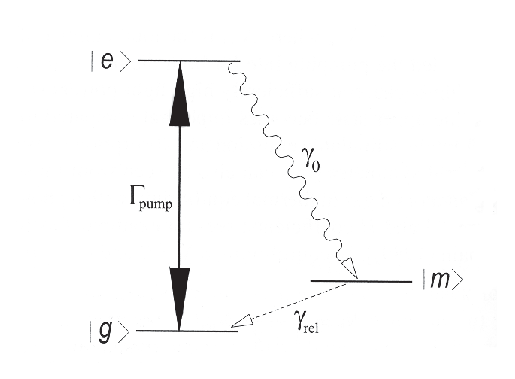
\includegraphics[width=4in]{figures/pumping.eps}
\caption{\small{Three level system with optical pumping rate $\Gamma_{pump}$}}
\label{fig:pumping}
\end{center}
\end{figure}


\subsection{Rubidium System}

In this experiment, we consider an ensemble of rubidium atoms as an
optical pumping system. Rubidium is an alkali atom with a single
electron in its outer shell, and thus can be modelled as a
hydrogen-like system. Here, we take the outer $5^2S_{1/2}$ level as
the ground state and focus on the $D_1$ transition between the
$5^2S_{1/2}$ and $5^2P_{1/2}$ states. 

\subsubsection{Spin-Orbit and Hyperfine Splitting}
We use a natural abundance Rubidium cell for optical pumping, which
consists of $72\%$ $^{85}$Rb and $28\%$ $^{87}$Rb, so we are able to
investigate the properties of both isotopes. The energy level diagrams
are presented in Fig.~\ref{fig:8587levels}.


\begin{figure}[h]
\begin{center}
\subfigure[$^{87}$Rb energy spectrum]{\label{fig:edge-b}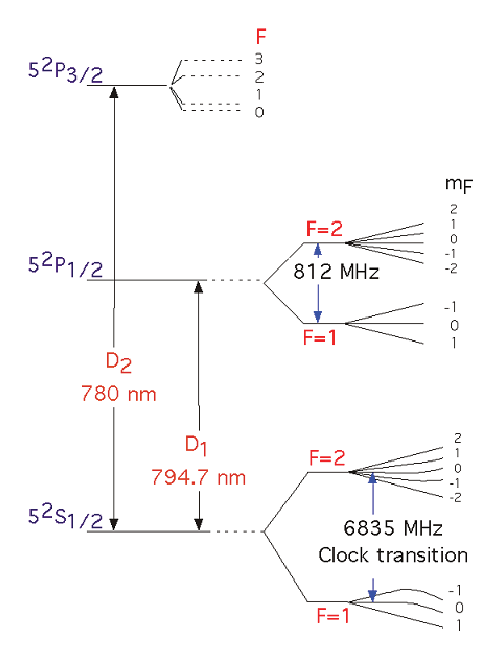
\includegraphics[height=3.5in]{figures/87levels.eps}}
\hspace{-1mm}
\vspace{-2mm}
\subfigure[$^{85}$Rb energy spectrum]{\label{fig:edge-a}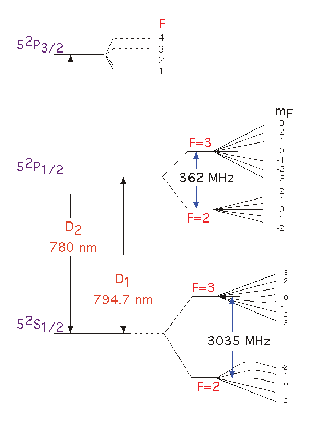
\includegraphics[height=3.5in]{figures/85levels.eps}}
\vspace{-2mm}
\caption{\small{The energy spectra of both isotopes of rubidium. Note the higher levels of degeneracy in the $^{85}$Rb system.}}
\label{fig:8587levels}
\end{center}
\end{figure}

There are several levels of splitting which occur in the rubidium atom. The
splitting of the $5^2P$ state into $5^2P_{1/2}$ and $5^2P_{3/2}$ is
due to spin-orbit coupling, \emph{i.e.}, the addition of the spin and
orbital angular momenta ($S$ and $L$, respectively) of the electrion
to create the total angular momentum $J$. As mentioned above, the
laser has been tuned to the $D_1$ line because of its better optical
pumping properties (Fig.~\ref{fig:8587levels}).

In addition, each total electron angular momentum level is further
split by the coupling of spins of the electron to the nucleus, a process known
as hyperfine splitting. This results in the distinct $F$ levels, where
$F = I + J$; $I$ is the spin of the nucleus and $J$ as above is the
total electron angluar momentum. Each pair of $F$ states in these
levels of rubidium are separated by a frequency shift on the order of
hundreds or thousands of MHz, allowing the tuning of the laser to a
particular transition (Fig.~\ref{fig:fluor}). For instance, we
chose to focus on the $^{85}$Rb $5^2S_{1/2}, F = 3$ to $5^2P_{1/2}, F
= 3$ transition for most of the experiment, because the density of the
$^{85}$Rb isotope is over twice as high, and the $3\rightarrow3$ line is
more easily separated from the neighboring transitions.

\begin{figure}[h]
\begin{center}
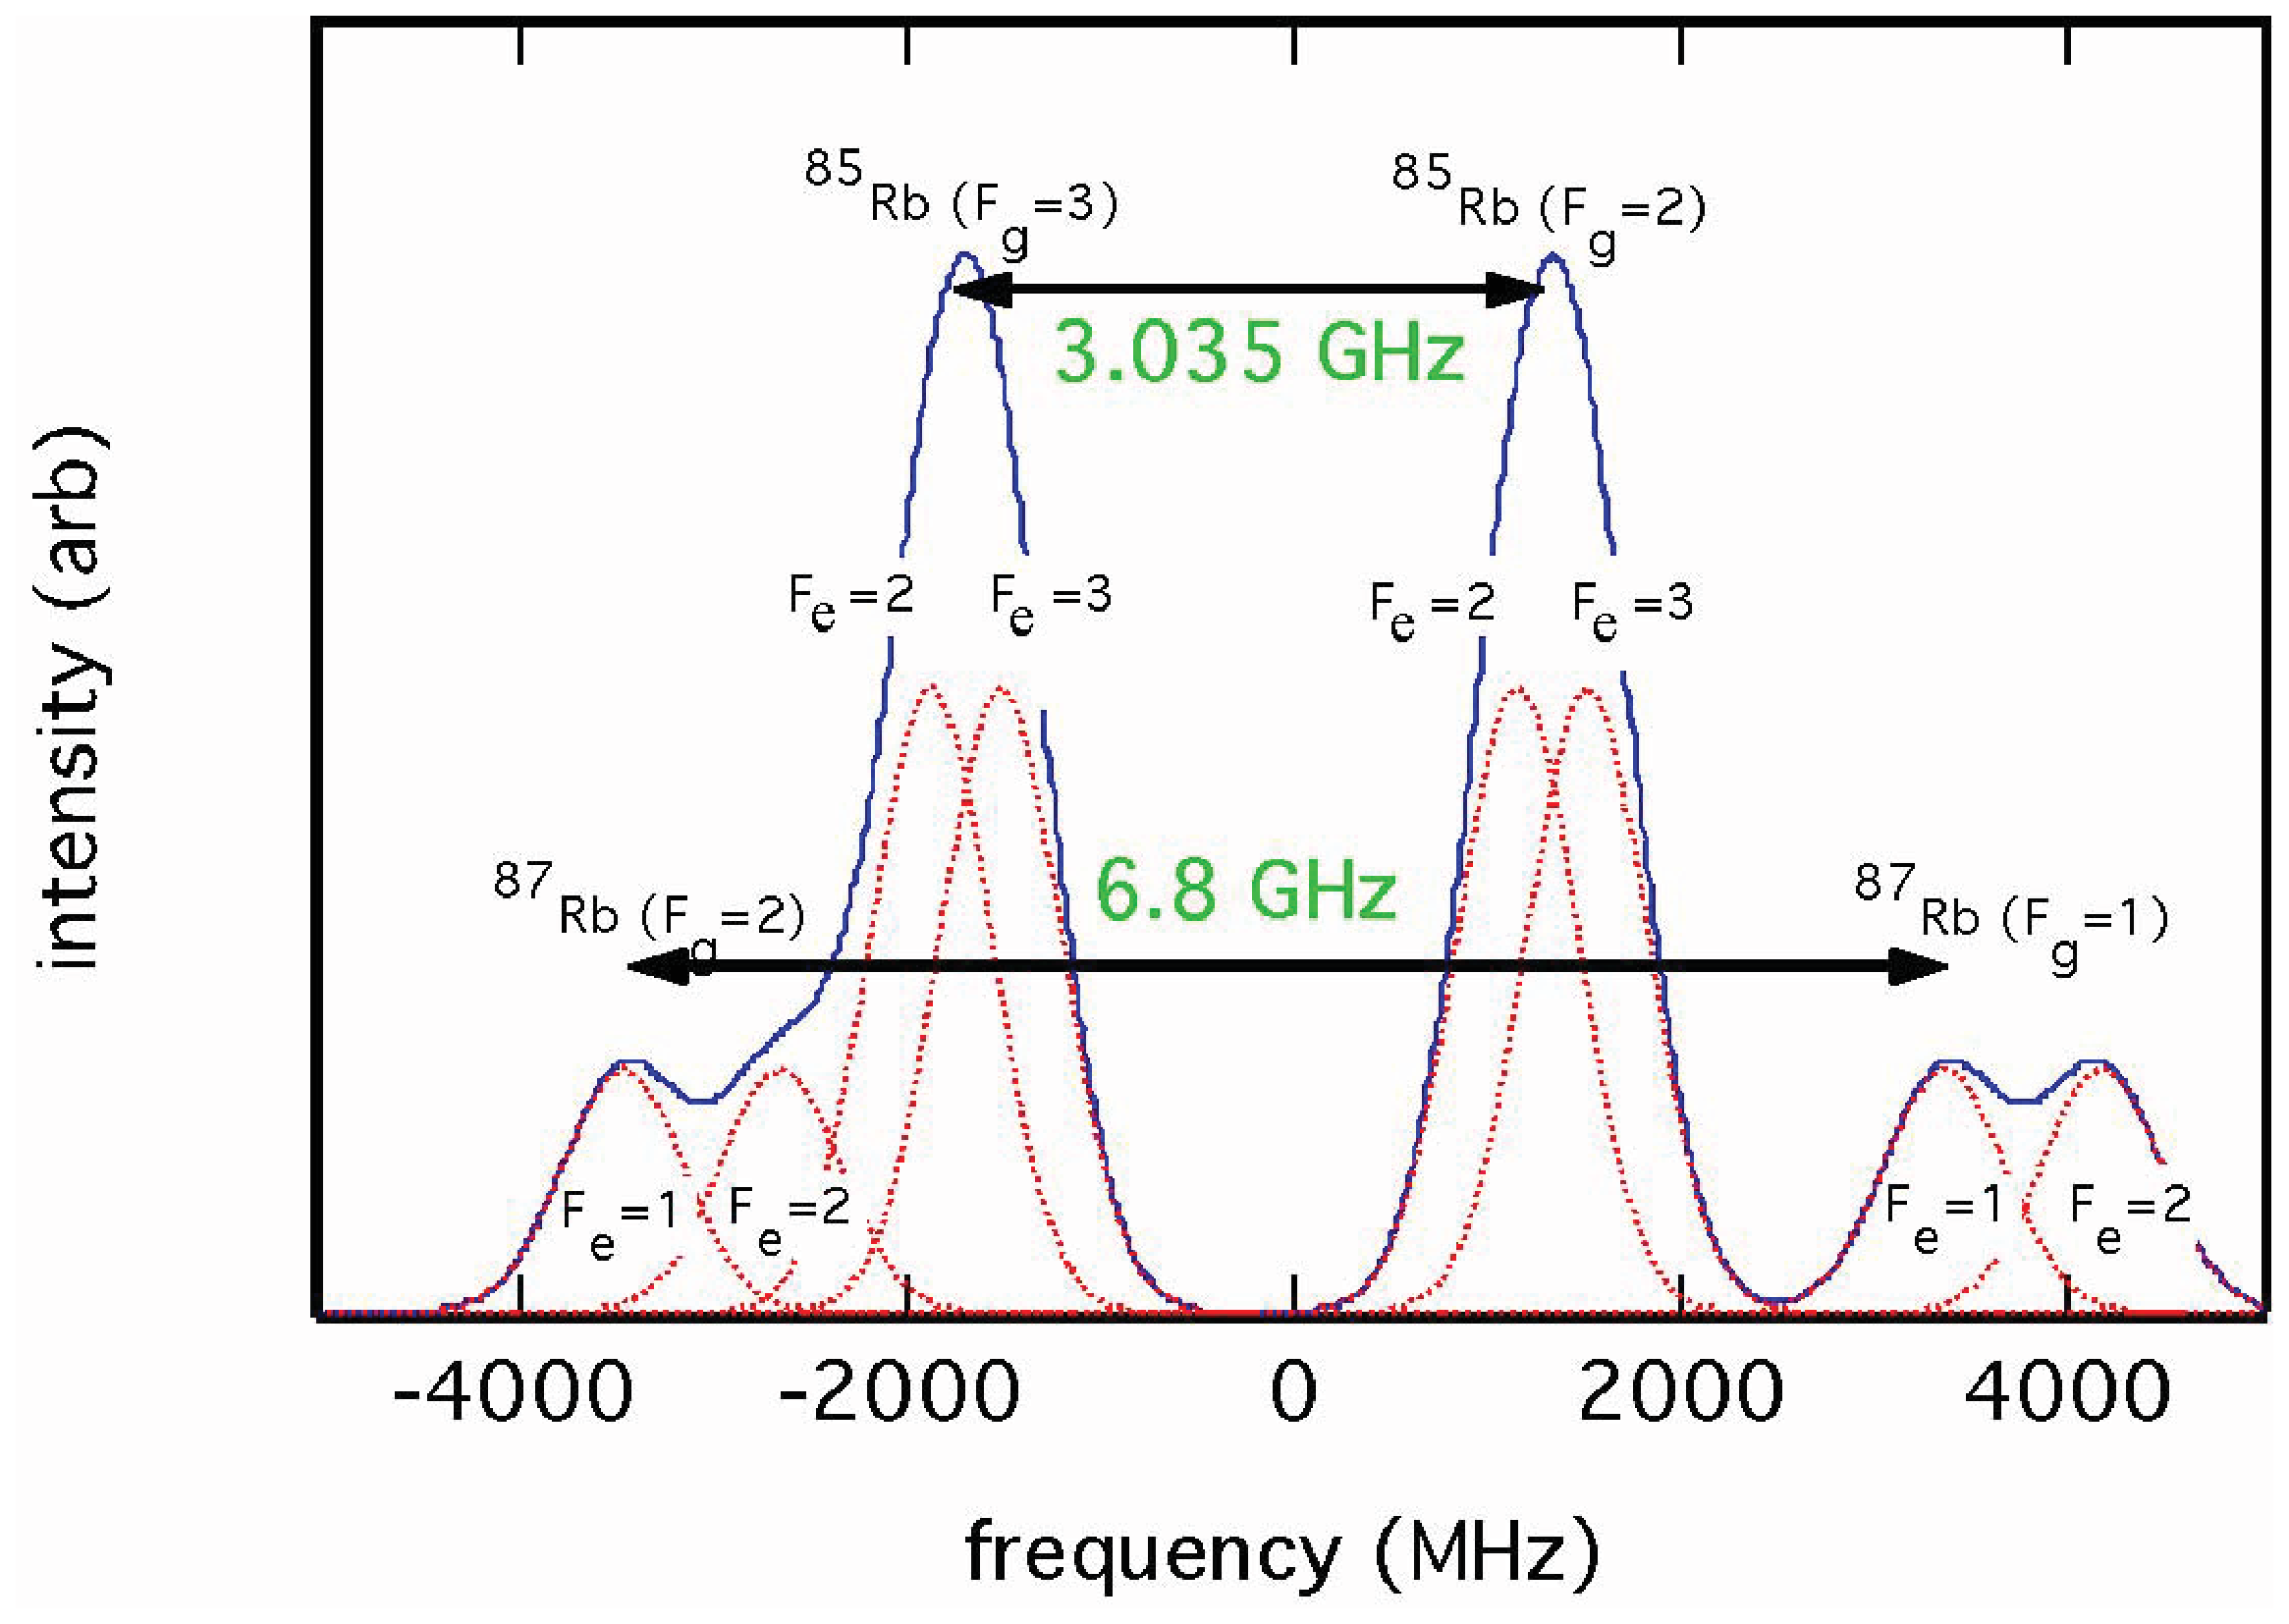
\includegraphics[height=3in]{figures/fluorescence.eps}
\caption{\small{Fluoresence spectrum of natural abundance rubidium. The $x$-axis is a relative measure of frequecy, with $0$ being the $D_1$ transition frequency. The dashed red line represents the fluorescence from individual transitions, and the blue line is the combined intensity.}}
\label{fig:fluor}
\end{center}
\end{figure}


\subsubsection{Zeeman Effect}
Further splitting occurs due to the Zeeman effect, where the degenerate
magnetic sublevels are split via an application of a uniform magnetic
field. For weak fields, the splitting is directly proportional to $B$,
the magnetic field amplitude and the magnetic dipole moment. The
change in the energy is given by

\begin{equation}
\Delta E = g_F\mu_B B m_F
\label{eqn:zeeman}
\end{equation}

where $\mu_B = \frac{e\hbar}{2m_e}$ is the Bohr magneton, $B$ is the
$z$-projection of the magnetic field, and $m_F$ is the spin projection
in the $z$ direction of the total angluar momentum of the atom
\cite{budker}. The qualitative dependence of these splittings on
magnetic field amplitude can be seen in Fig.~\ref{fig:8587levels},
where the energy split between initally degenerate levels increases
with magnetic field.

\subsubsection{Application to Optical Pumping}

In our experiment, the different splittings of the rubidium levels are
used as an effective 3-level system, as described in
section~\ref{opticalpumping}. Although there are many levels in a
rubidium atom, it is valid to approximate the system as composed of
only the $5^2S_{1/2}$ and $5^2P_{1/2}$ sublevels if the laser is on
the $D_1$ line, as it does not interact with the states which are not on
resonance. We treat the set of $5^2S_{1/2}$ levels as the ground
states, and $5^2P_{1/2}$ as the excited states. 

By applying a uniform magnetic field, the magnetic sublevels are
split, and one can act as the metastable `dark' state $|m\rangle$
necessary for optical pumping as follows: if $\sigma_+$-polarized
laser light is applied to the atom, then the only allowed transitions
to an excited state are those with $\Delta m_F = +1$.
(Fig.~\ref{fig:rbpump}). In the case of a $F = 1$ to $F = 1$
transition, for instance, the ground state with $m_F = 1$ is the
`dark' state because it cannot absorb $\sigma_+$ light. However, atoms
do get excited from the $m_F = -1, 0$ states, and then spontaneously
decay into all three ground states. Therefore, there is an overall
positive rate of atoms going into the `dark' state, increasing
transmission of laser light and creating the conditions of optical pumping, as desired. 

\begin{figure}[h]
\begin{center}
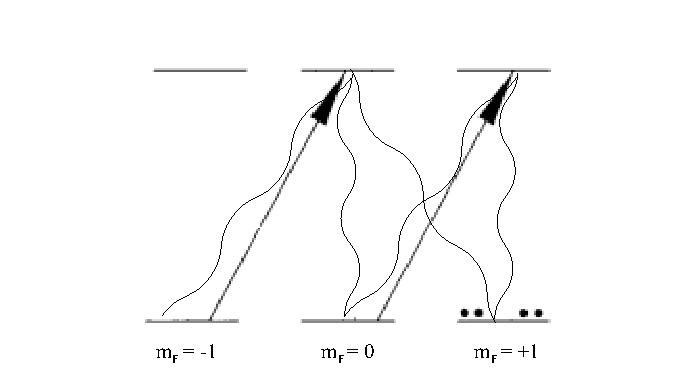
\includegraphics[height=2.5in]{figures/rbpump.eps}
\caption{\small{Effects of optical pumping on the $1\rightarrow 1$
    transition with $\sigma_+$ light on the populations of the ground
    state Zeeman levels. Due to quantum exclusion rules, the ground
    $m_F = +1$ state is `dark' to the laser, and atoms get
    preferentially pumped into this state.}}
\label{fig:rbpump}
\end{center}
\end{figure}


\subsection{Magnetic Interactions}

In order to study the properties of the rubidium atoms, such as the
g-factor, we introduce a magnetic field transverse to the $z$
direction as established by the laser and uniform magnetic field. This
field is introduced at a radiofrequency on the order of the Zeeman splittings,
coupling the dark state with the remaining ground states. 

\subsubsection{Rabi Oscillations}\label{rabioscillations}

For a two-level system with ground state energy $E_2$ and excited
state energy $E_1$, the application of a periodic perturbation of the
form $V(t) = V_0e^{i\omega t}$ with a relaxation (damping) term
proportional to a constant $\Gamma$, the time dependence of the
population of the upper state is given by

\begin{equation}
P(t) = \frac{(2V_0)^2e^{-\Gamma t/2}}{(2V_0)^2 +\Delta^2 + \Gamma^2/4}\sin^2(\frac{t}{2}\sqrt{(\Delta + \Gamma/2)^2 + (2V_0)^2}) \label{eqn:rabi}
\end{equation}

Here, $\Delta = \omega - \omega_0$ is the detuning, with $\omega_0 =
(E_1 - E_2)/\hbar$ the separation between the upper and lower state of
the system, and $\omega$ the frequency of the periodic
perturbation. $\Gamma$ is the natural decay rate of the population in
the excited state \cite{budker}.

This gives the general behavior of a driven, damped optical system. In
the case of a three level system, it is useful to make the
approximation of a small radiofrequency perturbation on top of the pumping
system. In that case the logic of the above discussion applies. Note
also that the peak amplitude of these oscillations occurs when
$\Delta\approx0$, \emph{i.e.}on resonance.


\subsection{Rate Equations}\label{rateequations}

Referring to Fig.~\ref{fig:pumping}, we can write down the rate equations
of the three level system:

\begin{eqnarray}
\frac{dN_g}{dt} &=& -\Gamma_{pump}N_g + \gamma_{rel}N_m\\
\frac{dN_e}{dt} &=& +\Gamma_{pump}N_g - \gamma_{0}N_e\\
\frac{dN_m}{dt} &=& +\gamma_{0}N_e - \gamma_{rel}N_m
\end{eqnarray}

where $N_g, N_e$, and $N_m$ are the populations of states
$|g\rangle$,$|e\rangle$, and $|m\rangle$, respectively.

To obtain the steady state result, we set the time derivates of the
populations to zero. With the assumption that $\gamma_{rel}<<
\gamma_0$ (as the transition from the metastable to the ground state
is a forbidden dipole transition, the rate is much slower), we solve to get 

\begin{equation}
N_e = \frac{\kappa}{1+\kappa}\frac{\gamma_{rel}}{\gamma_{0}}N_{tot}
\end{equation}

where $\kappa = \frac{d^2\mathcal{E}_0^2}{\gamma_0\gamma_{rel}}$ is
the laser light saturation parameter, with $d = \langle e|d|g\rangle$
the dipole matrix element between the excited and ground state,
$\mathcal{E}_0$ is the electric field amplitude of the laser, and
$\gamma_0$, $\gamma_{rel}$ are as in Fig.~\ref{fig:pumping}.

In terms of the detuning $\Delta$ from resonance, we can write the fluorescence intensity as

\begin{equation}
I(\Delta) = \frac{\gamma_0^2/4}{\Delta^2 +(1+\kappa)\gamma_0^2/4}\kappa\gamma_{rel}N_{tot}
\end{equation}

which a Lorentzian profile with width

\begin{equation}
\gamma_m = \gamma_0\sqrt{1+\kappa} = \gamma_0\sqrt{1+\kappa_l\mathcal{E}_0^2}
\end{equation}

where $\kappa_l = d^2/(\gamma_0\gamma_{rel})$ is a constant that
characterizes the broadening of the natural linewidth $\gamma_0$ with
increased light intensity $\mathcal{E}_0^2$.



As we are assuming that the coupling between states $|e\rangle$ and
$|m\rangle$ is minimal, this derivation holds only in the limit of
very weak radiofrequency perturbations. In order to understand the behavior of the
radiofrequency system, we make the two level approximation of the the three level
system. Following the derivation in Yariv, we can consider the two
level system with energies $E_1$ and $E_2$ and perturbing Hamiltonian
$\mathcal{H}'$.

Then the rate equations governing the time evolution of the density matrix $\rho$ are 

\begin{eqnarray}
\frac{d\rho_{12}}{dt} &=& -\frac{i}{\hbar}(\mathcal{H}'_{21}(\rho_{11} - \rho_{22}) + (E_2 - E_1)\rho_{21}) \\
 &=& -i\omega_0\rho_{21} + i\frac{\mu}{\hbar}E(t)(\rho_{11} - \rho_{22})
\label{pump1}
\end{eqnarray}

where $\omega_0 = (E_2 - E_1)/\hbar$ and $-\mu E(t)$ is the pertubing
hamiltonian.

We also have

\begin{eqnarray}
\frac{d\rho_{22}}{dt} &=& -i\frac{\mu}{\hbar}E(t)(\rho_{21} - \rho_{21}^*)\\
\frac{d}{dt}(\rho_{11} - \rho_{22}) &=& 2i\frac{\mu}{\hbar}E(t)(\rho_{21} - \rho_{21}^*)
\label{pump2}
\end{eqnarray}

Now we introduce the relaxation times $T_1$ and $T_2$ by modifying Eqns \ref{pump1} and \ref{pump2} as follows \cite{yariv}:

\begin{eqnarray}
\frac{d\rho_{12}}{dt} &=& -i\omega_0\rho_{21} + i\frac{\mu}{\hbar}E(t)(\rho_{11} - \rho_{22}) - \frac{\rho_{21}}{T_2}\\
\frac{d}{dt}(\rho_{11} - \rho_{22}) &=& 2i\frac{\mu}{\hbar}E(t)(\rho_{21} - \rho_{21}^*) - \frac{1}{T_1}((\rho_{11} - \rho_{22}) - (\rho_{11} - \rho_{22})_0)
\label{pump3}
\end{eqnarray}

where $N(\rho_{11} - \rho_{22})_0$ is the population in the
equilibrium state - in this case, with optical pumping but no radiofrequency
field.

Assuming a harmonic perturbation potential with amplitude $V_0$ and
frequency $\omega$, we can again solve for the steady state by setting
the time derivatives to $0$. This gives the polarization as

\begin{eqnarray}
P = \frac{\mu^2\Delta N_0 T_2}{\hbar}V_0\left(\frac{\sin\omega t + (\omega_0 - \omega)T_2\cos\omega t}{1 + (\omega - \omega_0)^2T_2^2 + 4\Omega^2T_2T_1}\right)
\label{pump4}
\end{eqnarray}

where $\Omega = \mu V_0/2\hbar$. Eqn.~\ref{pump4}, when expressed in
terms of the power absorbed by the medium, gives 

\begin{equation}
g(\nu) = \frac{(\Delta\nu/2\pi)}{(\nu-\nu_0)^2 +(\Delta\nu/2)^2}
\label{eqn:gamma1}
\end{equation}


where $g(\nu)$ is the normalized lineshape corresponding to the power. again, the lineshape is Lorentzian, with natural linewidth $\Delta\nu = (\pi T_2)^{-1}$. Taking into account the saturation phenomena, we can rewrite the observed linewidth as a function of powerbroadening:

\begin{equation}
\Delta\nu_m = \Delta\nu\sqrt{1+\frac{\mu^2V_0^2T_2T_1}{\hbar^2}} = \Delta\nu\sqrt{1+\kappa_{rf}V_0^2}
\label{eqn:gamma1}
\end{equation}

where $\kappa_{rf}$ is now a measure of line broadening as a function of RF. 


\subsubsection{Time Constants}\label{timeconstants}

Of particuar interest to experiment are the different time constants
which emerge from the rate equations. 

The optical pumping time $\tau$ is defined as $\tau =
1/\Gamma_{pump}$, the time it takes to change the total magnetization
of the atomic ensemble from thermal equilibrium to the maximal
equilibrium value with the presence of an external electromagnetic
field. 

$T_1 = 1/\gamma_1$ is time constant of longitudinal relaxation,
i.e. the time that the diagonal elements of the density matrix
$\rho_{jj}$ return to the equilibrium in the absence of other
perturbations. There are several effects which contribute to the
relaxation rate, and they are assumed to add independently
\cite{vanier}:

\begin{equation}
\gamma_1 = \gamma_{1,se} + \gamma_{1,w} + \gamma_{1,bg} 
\label{eqn:gamma1}
\end{equation}

Here, $\gamma_{1,se}$ is the spin exchange relaxation rate,
$\gamma_{1,w}$ is the wall collision rate due to leaving the beam, and
$\gamma_{1,bg}$ is the rate due to buffer gas collisions
\cite{vanier}.

$T_1$ can be calculated by detemining the decay of the population
coherence ``in the dark'', that is with no optical pumping.

$T_2 = 1/\gamma_2$ is the time constant of transverse relaxation,
alternatively described as the time constant of coherence relaxation
of the off-diagonal density matrix elements $\rho_{ij}$. As for
$\gamma_1$, different effects contribute to the linewidth:

\begin{equation}
\gamma_2 = \gamma_{2,se} + \gamma_{2,w} + \gamma_{2,bg} 
\label{eqn:gamma2}
\end{equation} 
 
where the components are the $T_2$ counterparts of those in
Eqn~\ref{eqn:gamma1}.

As seen in section \ref{rateequations}, $T_2$ can be reconstructed
from calculating the natural linewidth of the RF resonance. This can
be done either by measuring a dependence of the broadened linewidth on
light intensity at low RF amplitude, or its dependence on RF amplitude
at low light intensity, in order to stay in one of the two
appoximation regimes treated above, and thus extrapolate to the
natural linewidth at $V_0 = \mathcal{E}_0 = 0$.

\subsection{Spin Exchange}\label{spinexchange}

A spin exchange process occurs when two particles transfer their spin orientations in a collision. \cite{bernheim}. Let $A$ and $B$ be two $^2S_{1/2}$
alkali atoms. Then a spin-exchange collision between the two atoms
can be represented by the equation

\begin{equation}
A(\uparrow) + B(\downarrow) \rightarrow A(\downarrow) + B(\uparrow)
\end{equation}

so the spin orientations of the two atoms are exchanged, while the
total spin is conserved \cite{happer}.  

The mechanism of spin exchange is one of the largest factors
contributing to the natural linewidth of the radiofrequency resonance ($T_2$ time) and
the $T_1$ time \cite{vanier}. In addition, spin exchange is a valuable
technique of studying the properties of an atom or particle for which
a direct optical particle procedure is much more difficult.

In this experiment, we use the spin exchange mechanisms between
$^{85}$Rb and $^{87}$Rb in order to study the contribution of spin
exchange collisions to the inherent radiofrequency linewidth of the two isotopes
(Eqn.~\ref{eqn:gamma2}).

\subsection{Inhomogeneous Broadening}\label{inhomogeneousbroadening}

In Section~\ref{rateequations} above, the homogeneous broadening
mechanisms contributing to the line width of $\gamma_2$ and
$\gamma_1$. In the case of homogeneous broadening, the assumption is
made that the interaction of the electromagnetic fields with the
individual magnetic moments of the atoms that has the same features
for every member of the atomic ensemble. In this case, every sample of
atoms is representative of the average behaviour of the entire system
\cite{vanier}. 

In the case of inhomogeneities in the system, further broadening can
occur. The most common causes of inhomogeneous broadening relevant to
our optical pumping experiment are Doppler effects and magnetic field
inhomogeneities. The additional broadening $\nu_D$ due to the Doppler effect
is given by

\begin{equation}
\nu_D = 2\nu_0\sqrt{\frac{2 k T}{M c^2}\ln{2}}
\end{equation}

where $\nu_0$ is the unbroadened linewidth, $k$ is Boltzmann's
constant, $T$ is temperature of the gas and $M$ is the atomic mass of
the gas \cite{yariv}. For the quantities in our experiment, the
Doppler linewidth addition is $6$ orders of magnitudes smaller than
the natural width, so it is not a detectable effect for the present
conditions.

The effect of magnetic field inhomogeneity is much more difficult to
express analytically, because it depends on the nature of the
inhomogeneities. Generally, the overall line shape can be expressed as
a sum of individual homogeneously broaded lines, $i.e.$ Lorentzians,
with a range of center frequencies
(Fig~\ref{fig:inhomo})\cite{vanier}. The broadening occurs because
different samples of atoms will effectively experience different
amplitudes of the magnetic field due to the inhomogeneity,
resulting in a range of Zeeman splittings and a range of center
frequencies for the ensemble's resonance.

\begin{figure}[h]
\begin{center}
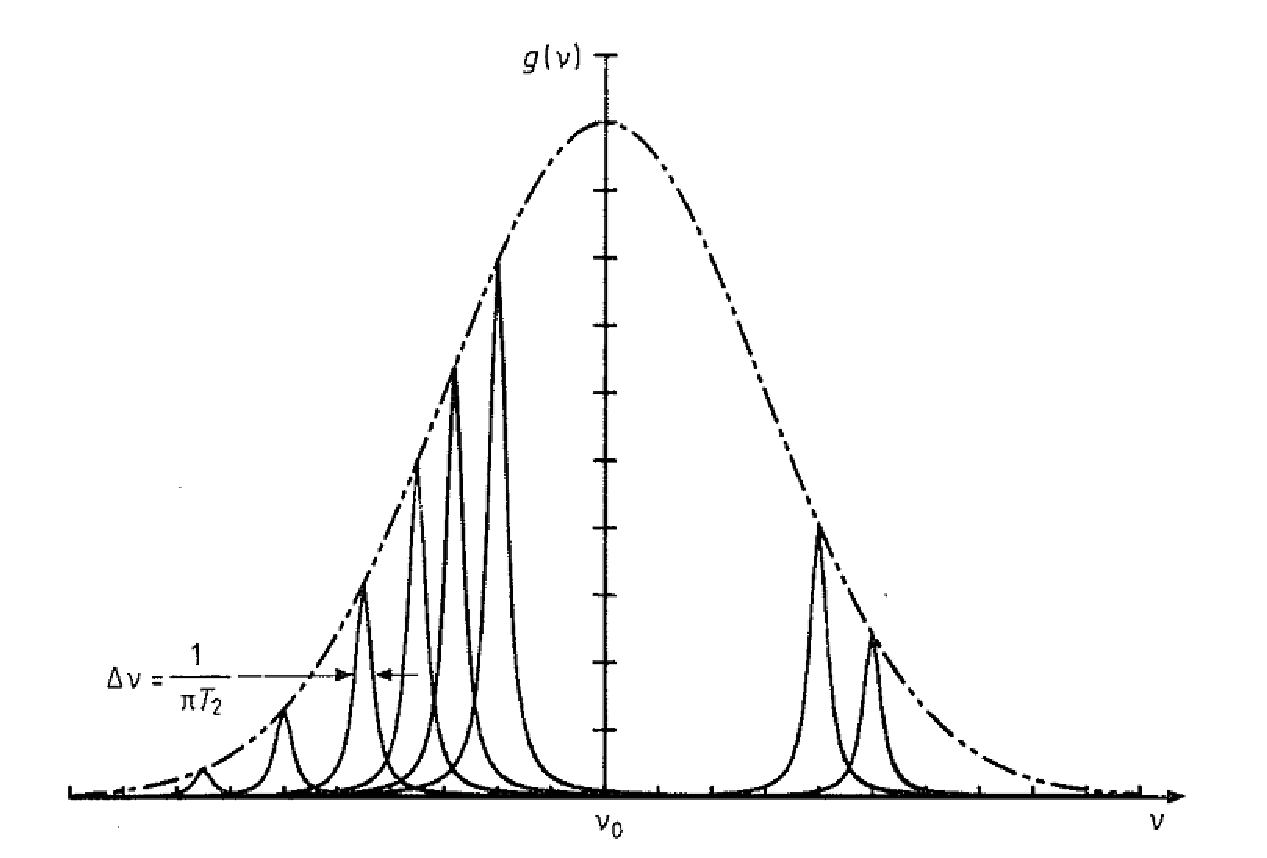
\includegraphics[height=3in]{figures/inhomogeneous.eps}
\caption{\small{In the event of inhomogeneities in the system (\emph{e.g.} in the uniform magnetic field), the overall linewidth of the radiofrequency resonance becomes broadened. The general form of the broadening is shown above, where each portion of the population of atoms experiences a different B field amplitude and has a different center frequency.}}
\label{fig:inhomo}
\end{center}
\end{figure}